\newpage
\section{Design Pattern}
\label{sec:pattern}

In questa sezione vengono analizzati i design pattern utilizzati.

\subsection{Strategy Pattern}
Quando una route è associata a più istanze dello stesso servizio, il sistema deve decidere quale usare per gestire ciascuna richiesta. 
Dato che non esiste un unico algoritmo ottimo per ogni scenario, è stato adottato il pattern \textbf{Strategy}.

Questo pattern permette di definire una famiglia di algoritmi, incapsularli in classi separate, implementando un'unica interfaccia \texttt{LoadBalancingStrategy}.
Questo li rende intercambiabili senza modificare il codice del \texttt{Client} che le utilizza.

\begin{figure}[H]
    \centering
    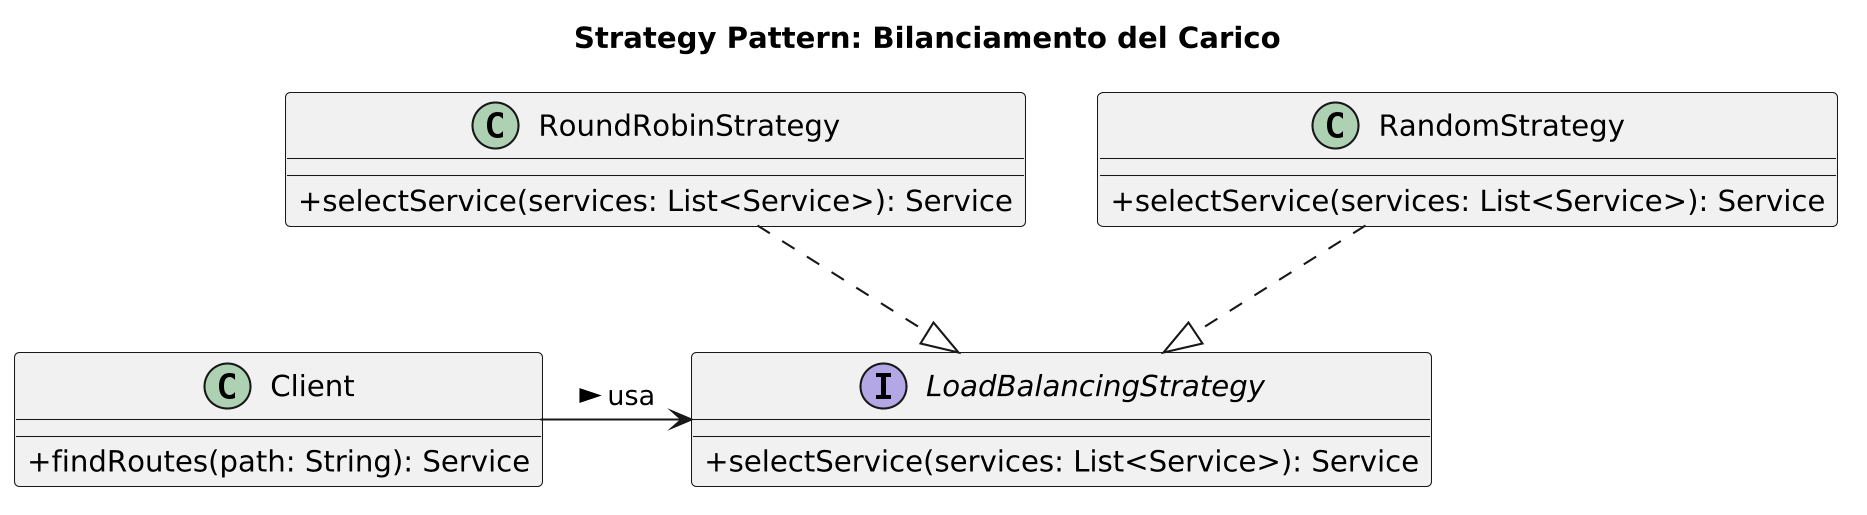
\includegraphics[width=\textwidth]{Images/design/strategy_pattern.png}
    \caption{Class Diagram ridotto per mostrare lo Strategy Pattern}
    \label{fig:strategy}
\end{figure}

\begin{java}[Implementazione Design Pattern]
public interface LoadBalancingStrategy {
    Service selectService(List<Service> services);
}

public class RoundRobinStrategy implements LoadBalancingStrategy {
    private final AtomicInteger counter = new AtomicInteger(0);

    @Override
    public Service selectService(List<Service> services) {
        int index = counter.getAndIncrement() % services.size();
        return services.get(index);
    }
}

public class RandomStrategy implements LoadBalancingStrategy {
    private final Random random = new Random();

    @Override
    public Service selectService(List<Service> services) {
        return services.get(random.nextInt(services.size()));
    }
}

public class Client implements Runnable {
    public Service findRoutes(String path) {
        for (Route r : ConfigurationManager.getInstance().getRoutes()) {
            if (r.getPath().equals(path)) {
                LoadBalancingStrategy strategy =
                    ConfigurationManager.getInstance().getLoadBalancingStrategy();
                return strategy.selectService(r.getService());
            }
        }
        return null;
    }
}
\end{java}

\subsection{Singleton Pattern}
La configurazione delle route viene letta una sola volta all'avvio dell'applicazione, ma è condivisa da tutti i thread \texttt{Client} generati per servire le richieste conteporaneamente. 
Per evitare di ricaricare più volte il file YAML e per garantire che tutti i thread usino sempre la stessa configurazione, è stato applicato il pattern \textbf{Singleton} alla classe \texttt{ConfigurationManager}.
Il costruttore privato impedisce la creazione di istanze al di fuori della classe stessa, mentre il metodo statico \texttt{getInstance()}, sincronizzato per essere sicuro anche in un contesto multi-thread, garantisce che la configurazione venga caricata al primo utilizzo e riutilizzata per tutta la durata dell'esecuzione.

\begin{java}[Implementazione Design Pattern]
public class ConfigurationManager {
    private static ConfigurationManager instance;

    private final Config config;
    private final LoadBalancingStrategy loadBalancingStrategy;

    private ConfigurationManager() {
        this.config = loadYamlConfig();
        this.loadBalancingStrategy =
            LoadBalancingStrategyFactory.create(config.getStrategy());
    }

    public static synchronized ConfigurationManager getInstance() {
        if (instance == null) {
            instance = new ConfigurationManager();
        }
        return instance;
    }

    public List<Route> getRoutes() {
        return config.getRoutes();
    }

    public LoadBalancingStrategy getLoadBalancingStrategy() {
        return loadBalancingStrategy;
    }
}
\end{java}

\subsection{Factory Method Pattern}
Il campo \texttt{strategy} del file di configurazione è una stringa, che deve essere tradotta nell'oggetto \texttt{LoadBalancingStrategy} concreto corrispondente. 
Per evitare che questa logica di creazione nel codice del \texttt{ConfigurationManager} o del \texttt{Client}, è stato usato il pattern \textbf{Factory Method}, incapsulato nella classe \texttt{LoadBalancingStrategyFactory}.
Con questo pattern, per aggiungere un nuovo algoritmo è sufficiente creare una nuova implementazione di \texttt{LoadBalancingStrategy} ed estendere la factory con un nuovo caso, senza toccare altro.

\begin{figure}[H]
    \centering
    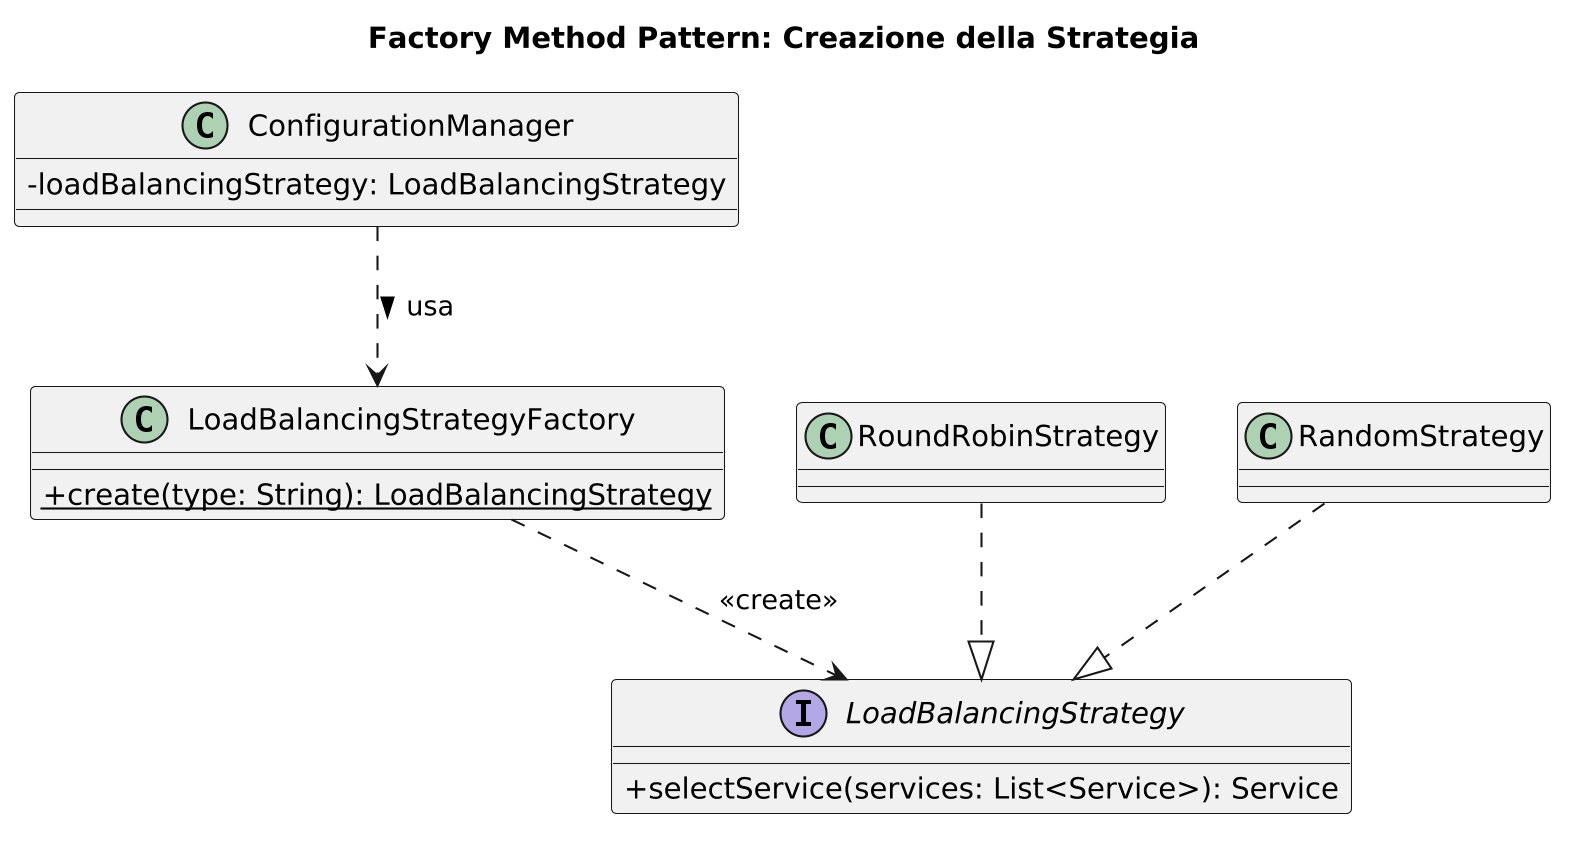
\includegraphics[width=0.9\textwidth]{Images/design/factory_pattern.png}
    \caption{Class Diagram ridotto per mostrare il Factory Method Pattern}
    \label{fig:factory}
\end{figure}

\begin{java}[Implementazione Design Pattern]
public class LoadBalancingStrategyFactory {
    public static LoadBalancingStrategy create(String type) {
        if (type == null) {
            return new RoundRobinStrategy();
        }
        switch (type.toLowerCase()) {
            case "random":
                return new RandomStrategy();
            case "round-robin":
            default:
                return new RoundRobinStrategy();
        }
    }
}
\end{java}

\subsection{Rispetto dei Principi SOLID}

La combinazione dei tre pattern descritti consente all'architettura di rispettare i principi SOLID:

\begin{itemize}
    \item \textbf{Single Responsibility Principle:} ogni classe ha una singola responsabilità ben definita:
      \begin{itemize}
        \item \texttt{Client} gestisce il ciclo di vita della connessione.
        \item \texttt{HttpRequest} rappresenta la richiesta.
        \item \texttt{ConfigurationManager} gestisce l'accesso alla configurazione.
        \item Ciascuna \texttt{LoadBalancingStrategy} implementa un solo algoritmo di selezione.
      \end{itemize}
    \item \textbf{Open/Closed Principle:} è possibile aggiungere nuove strategie di bilanciamento del carico creando nuove classi che implementano \texttt{LoadBalancingStrategy}, senza modificare altro.
    \item \textbf{Liskov Substitution Principle:} qualunque implementazione dell'interfaccia \texttt{LoadBalancingStrategy} può essere utilizzata al posto di un'altra senza alterare la correttezza di \texttt{Client}.
    \item \textbf{Interface Segregation Principle:} l'interfaccia \texttt{LoadBalancingStrategy} espone un solo metodo, evitando implementazioni inutili.
    \item \textbf{Dependency Inversion Principle:} \texttt{Client} dipende dall'astrazione \texttt{LoadBalancingStrategy} e non dalle sue implementazioni concrete.
\end{itemize}
